\LARGE{ \textbf {Лекция №12}}\\
\Large{ \textbf {Линейный дешифратор}}\\
Соединяет $ 2^n $ коньюкторов с $ n $ входами каждый коньюктор.\\
Синтез дешифратора с $ n = 2 $\\
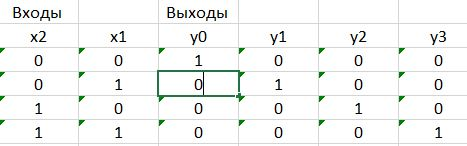
\includegraphics{42}\\
Для басиза И-НЕ\\
$ y_0 = \overline{ \overline{x_2} \overline{x_1}} $ \\
$ y_1 = \overline{ \overline{x_1} x_2}$\\
$ y_2 = \overline{ x_2 \overline{x_1}} $\\
$ y_3 =\overline{ x_2 x_1} $\\

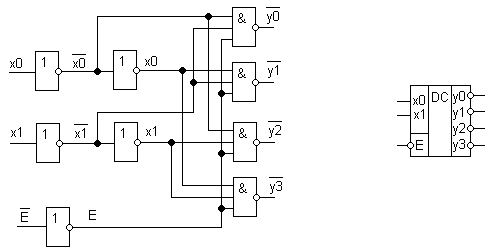
\includegraphics{43}\\
$T^{DC}_{zaderSR}= t_{zaderSR}^{NE} + t_{zaderSR}^{AND} $ \\
Недостатки\\
Гонки сигналов. Решение - стробирование.
Достоинства схемы\\
Быстродействие не зависит от разрядности схемы. (Нигде в формуле нет множителя)\\
Недостатки\\
С ростом разрядности дешифратора увеличивается количество входов у коньюктора, которое не может возрастать неограниченно.\\

Если в последовательном каскаде использовать И-НЕ, то получается дешифратор с инверсными выходами.\\
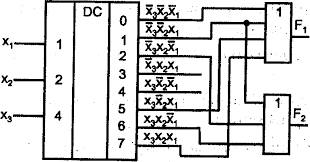
\includegraphics{44}\\

Парамидальный дешифратор (медленный)\\
$ n = 4 \quad y = \overline{x_1} \overline{x_2} \overline{x_3} \overline{x_4} $\\
$ n = 4 \quad y = ((\overline{x_1} \overline{x_2}) \overline{x_3}) \overline{x_4} $\\
$T^{DC}_{zaderSR}= t_{zaderSR}^{NE} + (n-1) t_{zaderSR}^{AND} $ \\
где, $ n-1  $ - количество каскадов.\\
С ростом разрядности  падает быстродействие дешифратора. Стробирование необходимо.\\

Ступеньчатые дешифраторы \\
$ n = 4 \quad y = (\overline{x_1} \overline{x_2}) \cdot (\overline{x_3} \overline{o_4}) $\\
где, $  (\overline{x_3} \overline{o_4}  $ - ступень.
n входов дешифратора разделяется на  группы по $ n/2  $  переменных $ x$ , если n- четное.\\
Для нечетного n  $ \frac{n+1}{2} \quad \frac{n-1}{2} $\\
В каждой группе реализуется линейный дешифратор и это состовляет 1 ступень дешифрации.\\
Затем по матричной схеме реализуется 2 ступень дешифрации, которая позволяет получить окончательный результат дешифрации.\\
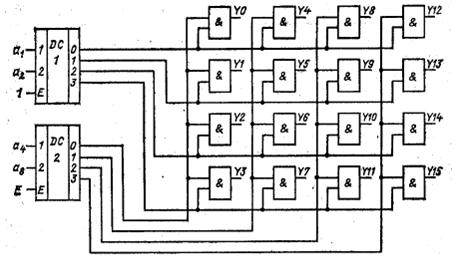
\includegraphics{45}\\

Для построения дешифратора большой разрядности используют ступеньчаиые дешифраторы.

Наращиваение дешифраторов\\

Для избежания гонок сигналов присутствует стробирующий вход  часто в дешифраторах бывает несколько стробирующих входов , например 2,
так как стробирующий вход может быть использован для наращивания дешифраторов, то есть получения дешифраторов большей разрядности.

СХЕМА.\\


Двоично-десятичный дешифратор.\\
Нееполный дешифратор, у которого 10 выходов.\\
 $y_0 = \overline{x_1} \overline{x_2} \overline{x_3} \overline{x_4} $\\
 $y_1 = \overline{x_1} \overline{x_2} \overline{x_3} x_4 $\\
 $y_8 = x_1 \overline{x_2} \overline{x_3} \overline{x_4} $\\
 $y_9 = x_1 \overline{x_2} \overline{x_3} x_4 $\\
Остальные выходы - 10-15 не используются, т.е. в них можно поставить любое значение.\\

\Large{ \textbf {Шифраторы.}}\\
Выполняют функцию обратную операции дешифрации.\\
CD - coder\\
Полный  двоичный Дешифратор имеет $2^n$ входов и n выходов.\\
При подаче сигнала на 1 из входов шифратора на выходе формируется слово, являющееся двоичным эквивалентом.\\

Приоритет подразумевает, какой въод имеет предпочтение в сравнении с другими входами.
Как правило, приоритеты расставляются по возрастанию.
Т.е. если подадим на 1 и 9 входы "1", то шифратор обработает тот сигнал, который имеет больший приоритет.



\textbf {Мульитплексор}\\
MX или MUX.\\
Коммутатор логичиских(цифровых) сигналов, обеспечивающий передачу информации
по нескольким входам на 1 выход. Выбор входа осуществляется в соответсвии с постоянным адресным входом.

При наличии m адресных входов можно реализовать $ N = 2^m $ комбинаций адресных сигналов,
каждый их которых обеспечивает выобор одно из N входных сигналов.

Мультиплексоры часто и инверсными бывают.

Применяются\\
\begin{enumerate}
  \item Для построения коммутаторов цифровых сигналов.
  \item ПЗУ (Постоянные запоминающие устройства $ 2^n x 1 $ бит)
  \item Преобразование кодов (Например, паралелльного в последовательный) (Или кода с одним )
\end{enumerate}


Наращивание  мультиплексора или объединение\\
Для реализации инверсии сигналов нужны инверторы. Поэтому необходимо стробирование.\\

Применение мультиплексоров.\\
Так как каждму адресу соответсвует только один информационный вход,
то с помощью мультиплексора можно реализовать любые логические функции адресных сигналов.
Но такие функции будут обладать аппаратной избыточности.
Допустим 4-1, сложение по модулю 2.\\
$z_1=a_0 |z_2 =a_o | f$\\
0 0 0\\
0 1 1\\
1 0 1\\
1 1 0\\
$x_0 = 0 , x_1 = 1, x_2 = 1, x_3 = 0$\\
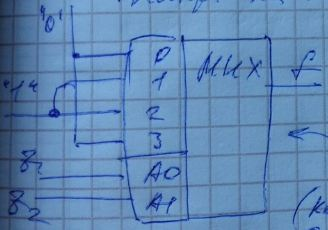
\includegraphics{56}\\
Это самый простой способ, когда кол-во функций соответсвует колву переменных.\\
Если значения выбирать не из $[0,1]$ , а из $[0,1,x_j,  \overline{x_j}]$ то на мульти с н входами можно реализовать
$x_j$ - один из аргументов функции.
Реализовать\\
$y = \overline{a}_0 \overline{a}_1 + a_2$\\
$x_0 = 1, x_1 = a_2, x_3= a_2,x_4= a_2$\\
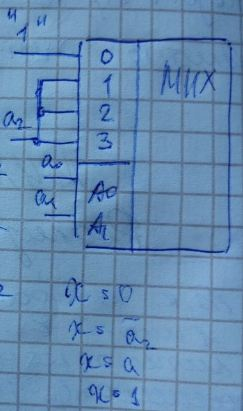
\includegraphics{55}
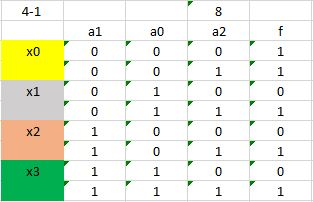
\includegraphics{54}\\

$y = x_0 \overline{a_1}\overline{a_0} + x_1 \overline{a_1} a_0 + x_2 a_1 \overline{a_0} + x_3 a_1 a_0$\\

Схеме необходимо стробирвоание. Кроме того стробирующий вход может использоваться дня наращивания мультиплексторов.
Задача: из 4-1 получить 8-1\\

Если $a_2 = 0$ , она запрещает работать второму мультиплексору.\\
Первый работает - он обеспечивают работу с 4 входами для него. В адресном пространстве $0xx$. \\
При этом будут присутсвовать гонки сигналов, потому что стробирующий вход занят.
Решение: либо 2 стробирующий вход, либо стробирование по последнему каскаду.
